\section{Website / front end}
\Diskussionspunkt{- Einleitung, Kurzzusammenfassung Problem Frontend}\newline

Die bisherige Anzeige der Wetterdaten basiert auf Adobe Flash, was nicht von allen Browsern unterstützt wird (siehe Fachmodul-Bericht). Die neue (2014) HTML5-Spezifikation ermöglicht es dynamische Grafiken zu erzeugen, die nativ von allen Web-Browsern dargestellt werden können.

%% ###################################################################################################
%%   Unterkapitel
%% ###################################################################################################
\subsection{Nutzungsanalyse der Webseite mittels Google Analytics}
Zuerst wurden die Zugriffsdaten auf die bestehende Webseite mittels Google Analytics analysiert. Als Zeitraum wurde das gesamte Jahr 2017 gewählt. Auf der bisherigen Webseite gab es zwei Unterseiten \textit{Wetter Tourismus} und \textit{Wetter Wassersport}, die sich aber nur gering voneinander unterscheiden z.B. in der Wahl der Einheit der Windgeschwindigkeit (km/h vs. kn). Die Zugriffsdaten sind in Abbildung \ref{img:google_mobile} dargestellt. Darin lässt sich erkennen, dass der Anteil an mobilen Geräten zwischen 50\% und 80\% beträgt. Dies wiederspiegelt den Trend zum mobilen Internet und zeigt wie wichtig die mobile Version einer Webseite ist. Dies geht soweit, dass sogar die mobile Seite als Ausgangspunkt für die Entwicklung der Homepage dient nach dem Designkonzept \textit{Mobile First}.

\begin{figure}[h!]
  \fbox{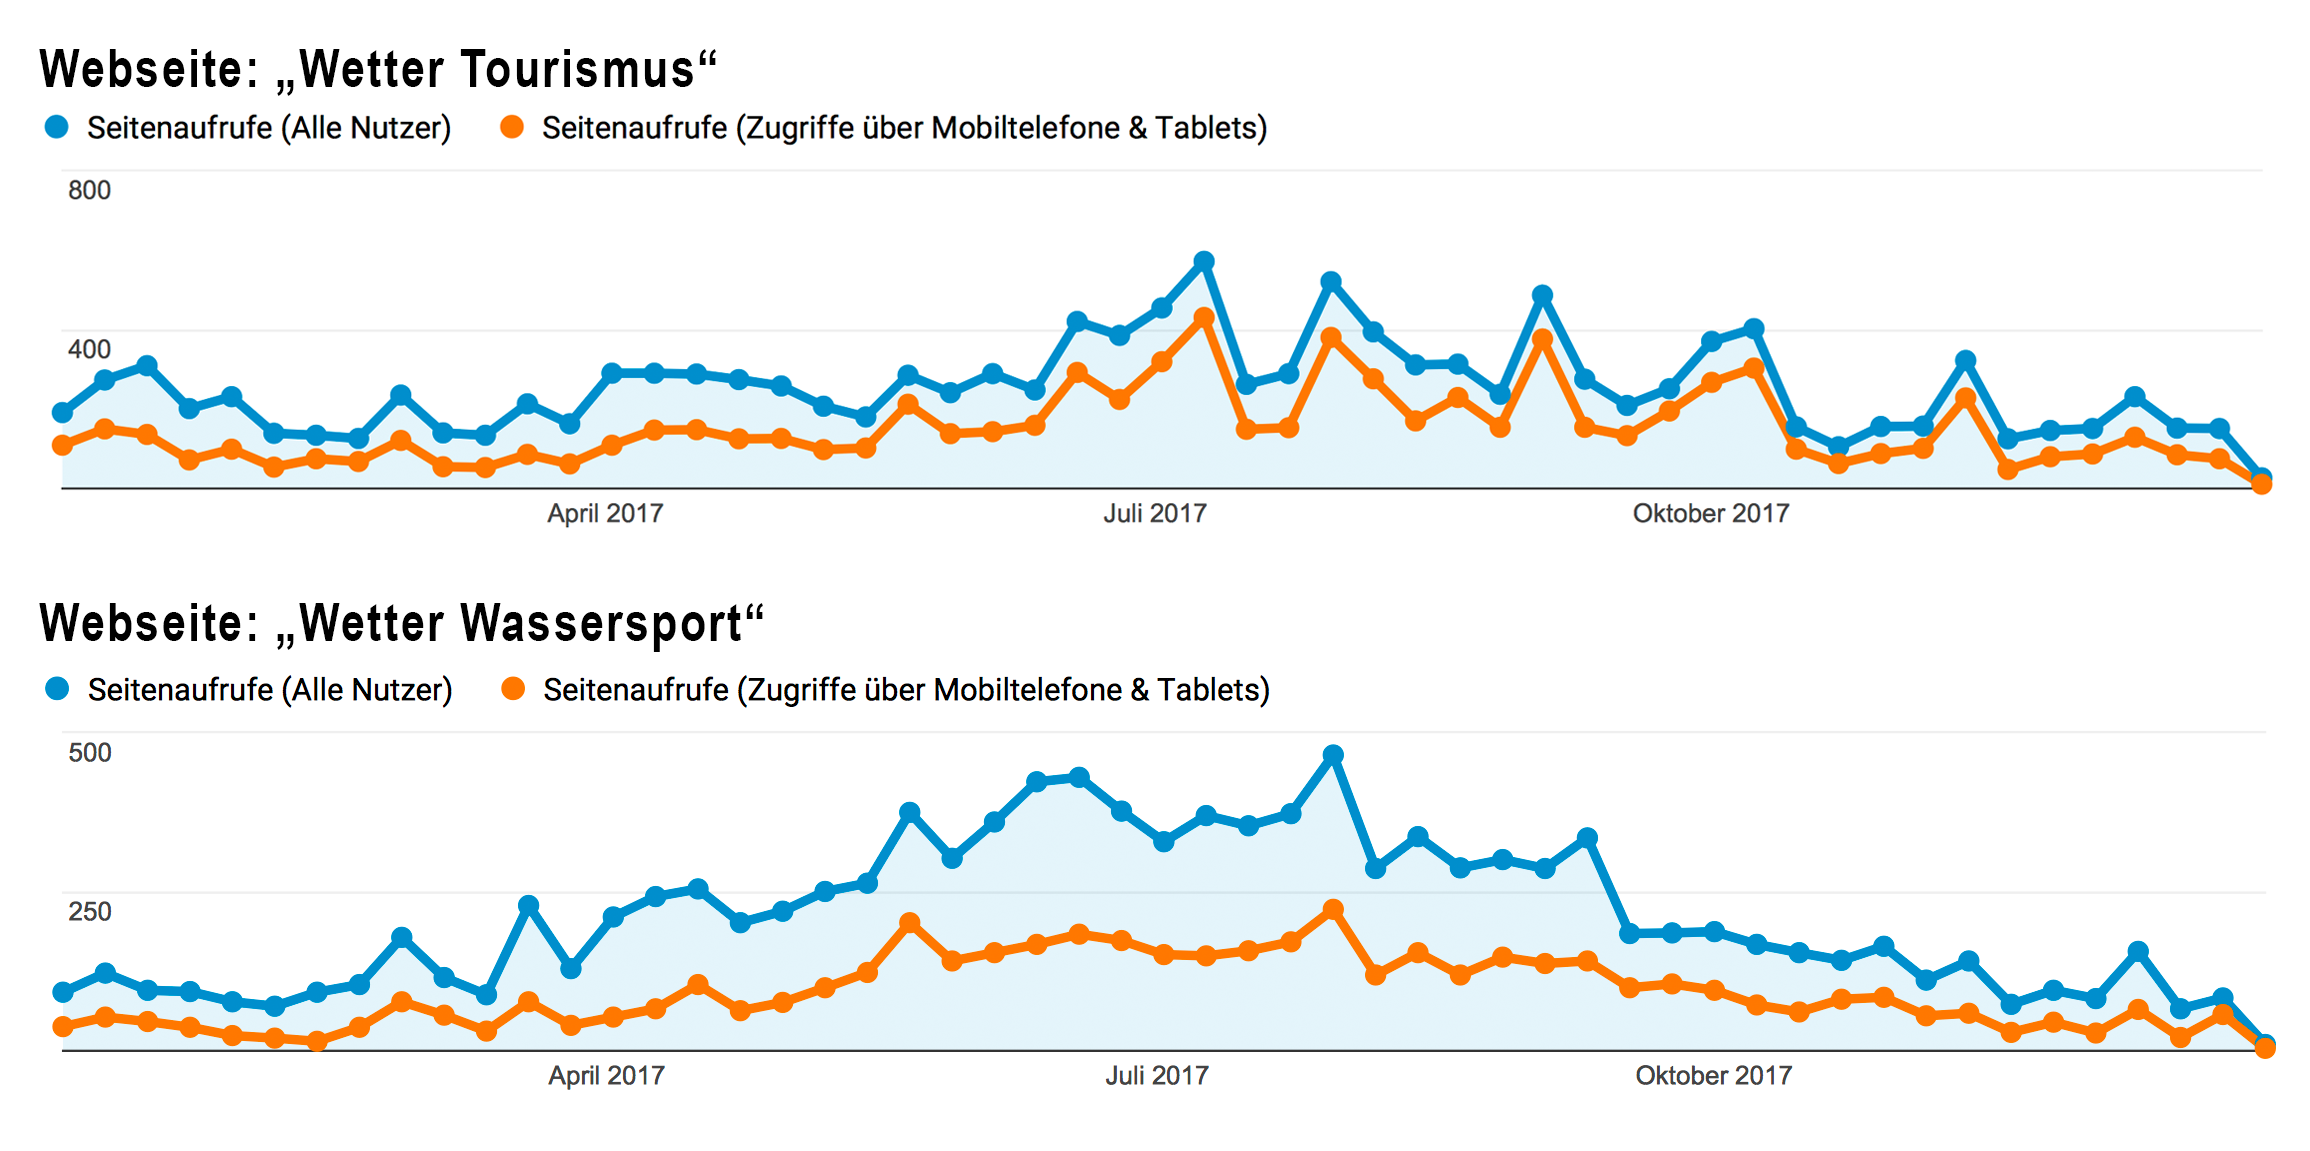
\includegraphics[width=\textwidth-2\fboxsep-2\fboxrule]{img/google_mobile}}
	\centering
	%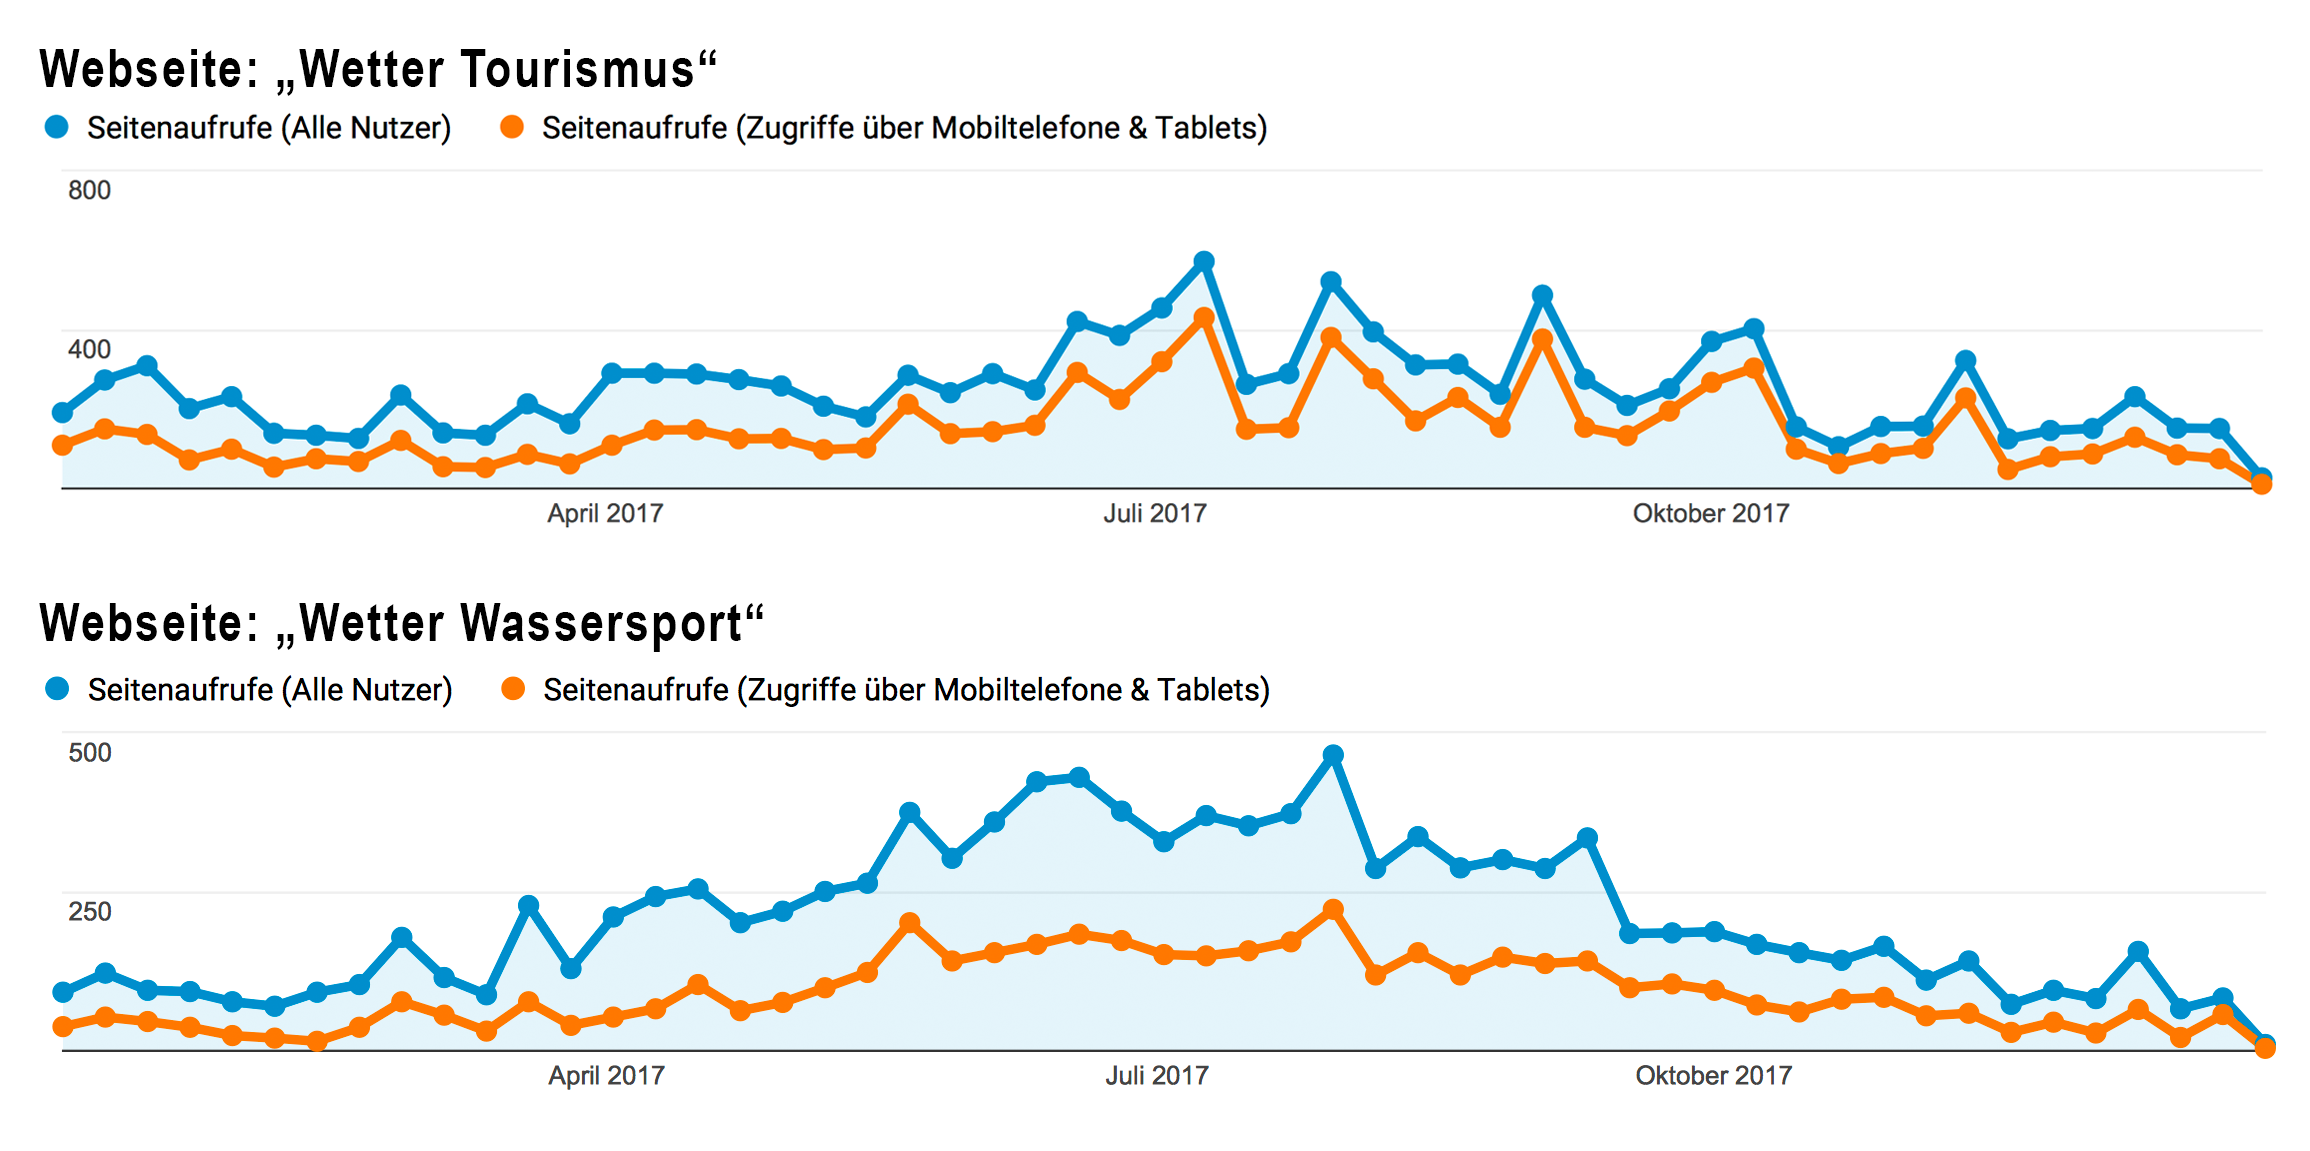
\includegraphics[width=1\linewidth]{img/google_mobile}
	\caption{Anteil der mobilen Zugriffe auf die Wetterwebseite}
	\label{img:google_mobile}
\end{figure}

Es lässt sich ebenfalls erkennen welche Browser am häufigsten verwendet werden und welches die beliebteste Seite der Website ist, wie in Abbildung \ref{img:google_browser} dargestellt.

\begin{figure}[h!]
	\centering
	\fbox{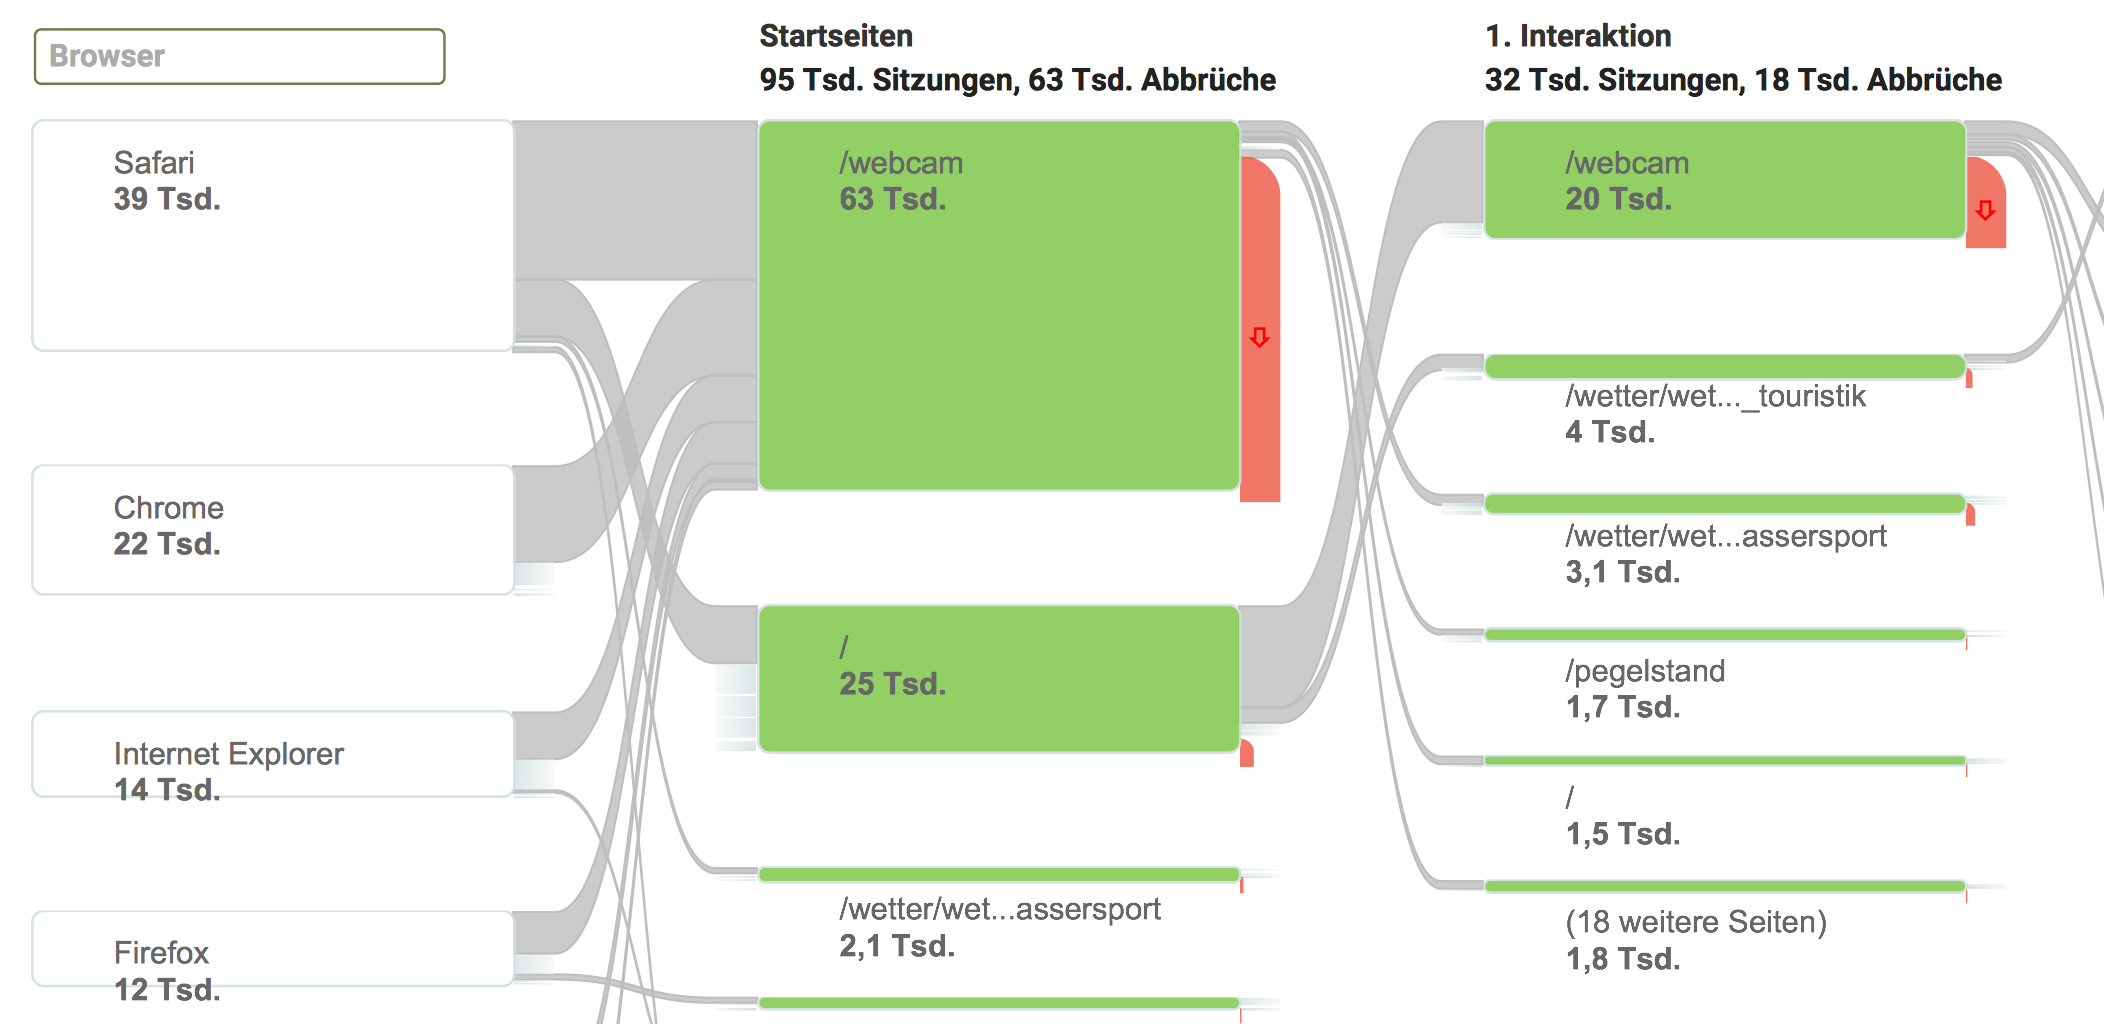
\includegraphics[width=\textwidth-2\fboxsep-2\fboxrule]{img/google_browser}}
	%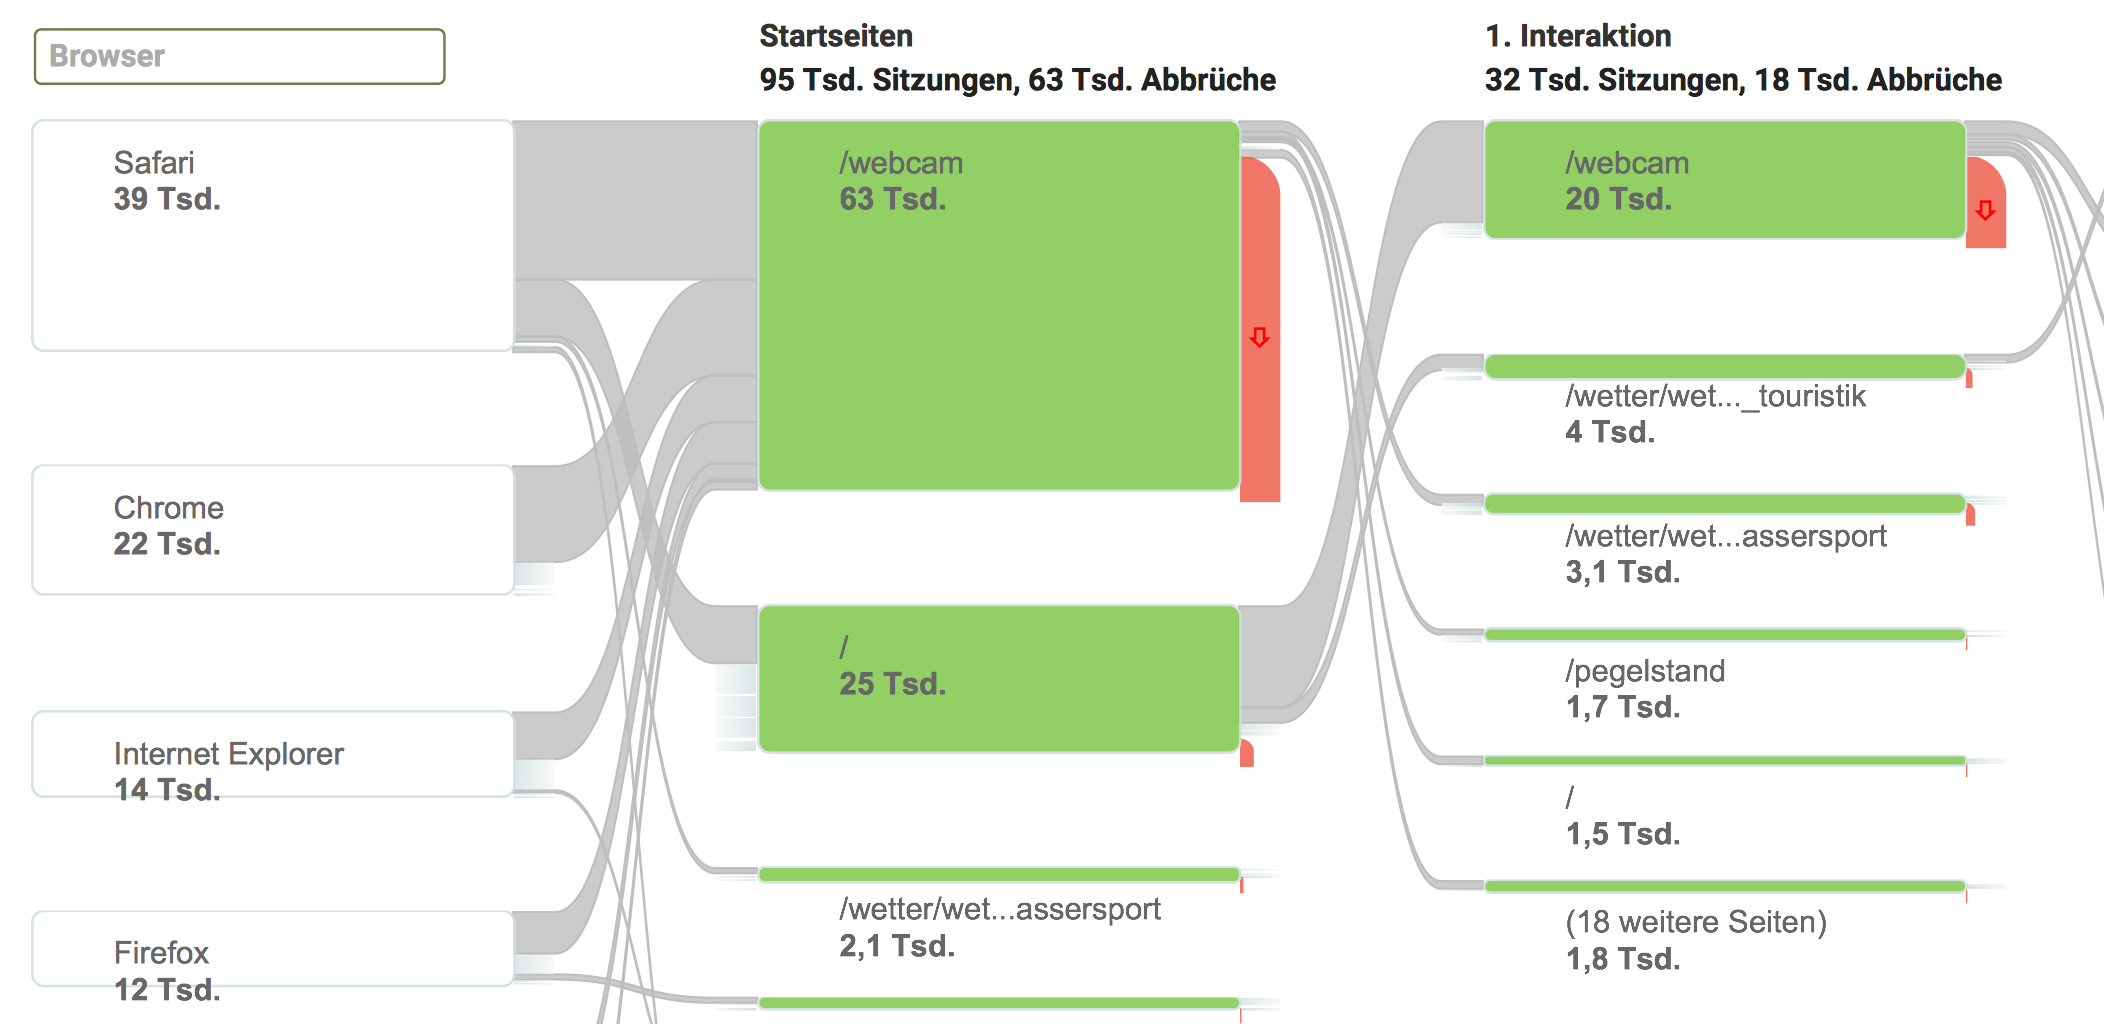
\includegraphics[width=1\linewidth]{img/google_browser}
	\caption{Verwendete Browser und Beliebtheit der Seiten}
	\label{img:google_browser}
\end{figure}


\Diskussionspunkt{- Wer sind die Nutzer}\newline
\Diskussionspunkt{- Warum Mobile First}\newline



\begin{itemize}
\item Ziel der Webseite definieren
\item Zielgruppe definieren
\item Ziel/Erwartungen der Zielgruppe erfassen
\item Wo wird die Infrmation gelesen
\item Was sind die Bedürfnisse der Benutzer
\item Scribbles erstellen
\item Wireframes erstellen
\end{itemize}

\subsubsection*{Ziel der Wetterstation-Webseite}
Interessierten, die wichtigsten Wetterparameter in leicht verständlicher Art zu präsentieren
\subsubsection*{Zielgruppe}
Touristen, Bevölkerung, Sportler, Interessierte
\subsubsection*{Erwartungen der Zielgruppe}
einfach und schnell verständliche Information
\subsubsection*{Scribbles}
Papierzeichnungen als erste Entwürfe
\subsubsection*{Wireframes}
Layout, gezeichnet mit balsamiq, ohne genaue Designangaben.


%% ###################################################################################################
%%   Unterkapitel
%% ###################################################################################################
\subsection{Darstellungskonzept / Nutzungskonzept}
\Diskussionspunkt{- Grafik mit den verwendbaren DIV}\newline
\Diskussionspunkt{- CSS-Framework, w3.css, chartist.css}\newline


\subsubsection{Randbedingungen durch CMS}
\Diskussionspunkt{- Aufbau openfile64}\newline
Die Webseite der Wetterstation ist mit dem Content-Management-System (CMS) \textit{Openfile64Light} der Firma Screenbox\footnote{ \url{https://screenbox.net/internet}}  erstellt. Dieses unterstützt grundsätzlich responsive Design. Das CMS gibt den Rahmen der Webseite vor. Spezielle Inhalte, wie zum Beispiel die Adobe Flash Animation, werden als sogenannte Applikationen behandelt und in die Seite eingebettet, gelb markiert in Abbildung~\ref{img:responsive}, links.

\begin{figure}[h!]
	\centering
	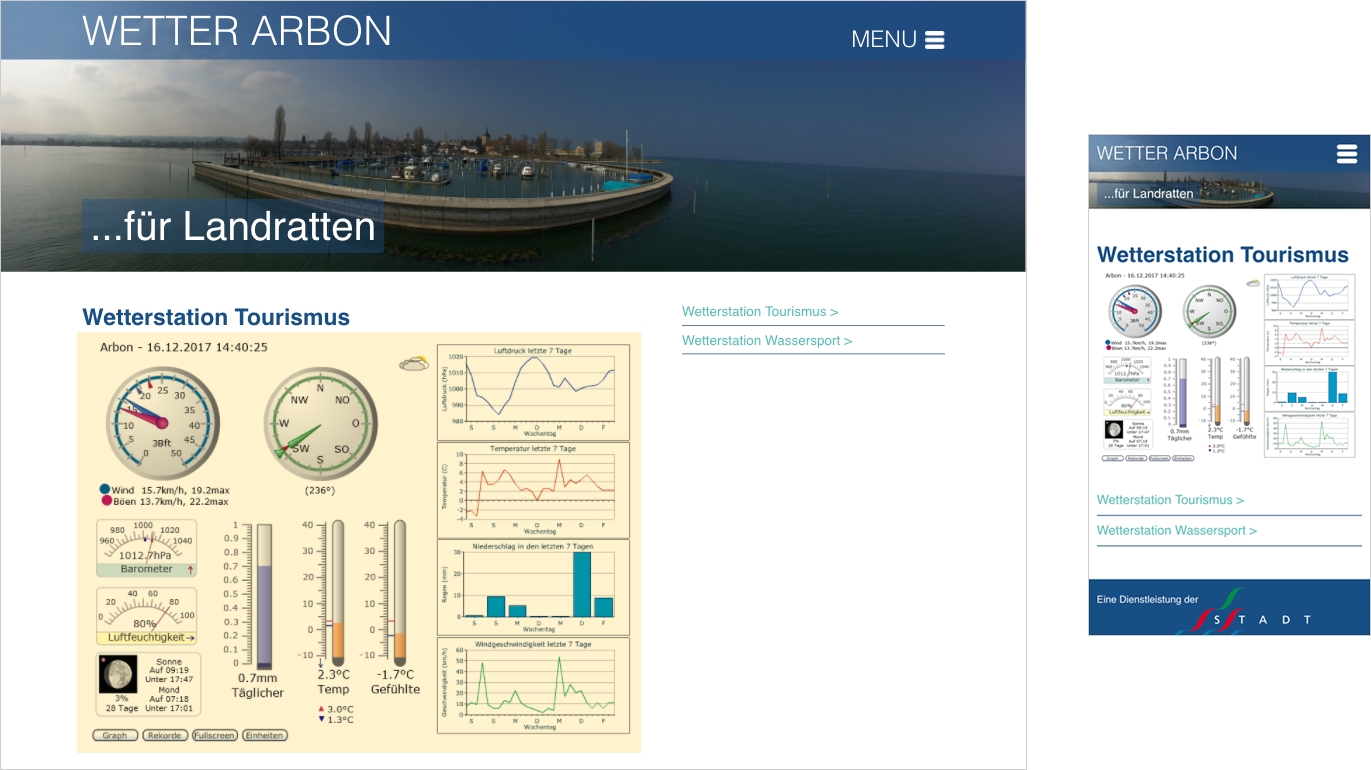
\includegraphics[width=1\linewidth]{img/responsive}
	\caption{Responsive Design: Vergleich Desktop und Mobile}
	\label{img:responsive}
\end{figure}



\subsubsection{Vorgehensweise, Design Konzept}
\Diskussionspunkt{- Responsive / Mobile First}\newline

Die Idee des Responsive Web Design wurde 2010 von Ethan Marcotte in einem Artikel \footnote{ \url{http://alistapart.com/article/responsive-web-design}} des Magazins A List Apart veröffentlicht. Hintergrund war, dass man nicht für jedes neue Gerät eine eigene Webseite erstellen musste. Marcotte schreibt von drei Faktoren, die ein responsive Design benötigt: Fluid grids, flexible images und media queries.

Fluid grids: Die Anordnung der Elemente passt sich dynamisch der Bildschirmgrösse an.
flexible images: Bilder haben keine feste Grösse sondern nutzen den ihnen zu Verfügung stehenden Platz optimal aus.
Media queries: sind die technische Basis für die beiden oberen Anforderungen.

Die "Mobile Web Best Practices" des W3C \footnote{ \url{https://www.w3.org/TR/mobile-bp}} empfiehlt, dass sämtliche Informationen, die in der Desktop-Version zur Verfügung stehen, auch von der mobilen Seite aufgerufen werden können (One Web Design).

Mobile First ist ein Designkonzept, bei dem die optimale Darstellung einer Website auf mobilen Endgeräten oberste Priorität hat. Bei Mobile First beginnt der Designer mit dem Mobile-Design und arbeitet sich dann schrittweise zur grösseren Desktop-Version vor. Vorteil: Da bei Mobile First die Grafiken und interaktiven Elemente schon zu Beginn für die Mobilversion optimiert werden, wird automatisch sichergestellt, dass diese auf jeder anderen Screengrösse auch umsetzbar sind.

Mobile First wurde von Luke Wroblewski 2009 das erste Mal vorgeschlagen. Es geht darum sich beim Designen einer Webseite zu erst auf die Kernfunktion zu konzentireren und diese zielgerichtet umzusetzen. Die benötigt eine vertiefte Analyse der Zielgruppe.

Vorgehen:






%% ###################################################################################################
%%   Unterkapitel
%% ###################################################################################################
\subsection{Grafische Darstellung der aktuellen Wetterdaten}
\Diskussionspunkt{- JS-Framework, justgage}\newline
\Diskussionspunkt{- code sniplet justgae, update}\newline
\Diskussionspunkt{- codesniplet update justgage}\newline
\Diskussionspunkt{- JS-Framework, justgage.js und raphael.js, jquery}\newline


\subsubsection{Gauges}
\Diskussionspunkt{- JS-Framework, justgage}\newline

-> erstellt eine svg-Grafik!!!!

\begin{lstlisting}[label=lst:gaugeJS,caption=Konfiguration der Gauge, language=JavaScript,mathescape, style=htmlcssjs]
    var temperature_gauge = new JustGage({
        id: 'temperature_gauge',
        value: initialValues.v1.data.temperature.value,
        min: -10,
        max: 40,
        symbol: "${^\circ}$C",
        title: 'Luft',
    });
\end{lstlisting}


\begin{lstlisting}[label=lst:gaugeHTML,caption=Container für die SVG-Grafik (Gauge), language=HTML5, style=htmlcssjs]
	<!-- Lufttemperatur -->
	<div class="w3-cell w3-col l2 m3 s6">
		<div class="w3-card">
			<div class="w3-container">
        		<p>Temperatur</p>
      </div>
			<div id="temperature_gauge" class="gauge"></div>
		</div>
	</div>
\end{lstlisting}

\subsubsection{svg-Grafiken mit Wertangabe}
\Diskussionspunkt{- verwendete Icon-Bibliothek}\newline


\subsubsection{Anzeige der aktuellen Sturmwarn-Situation}
\label{subsec:sturmwarnung}

% was ist der Sturmwarndienst und wie werden die verschiedenen Stufen dargestellt
Auf dem Bodensee gibt es einen Sturmwarndienst, der die Schiffsführer vor aufkommendem Sturm warnen soll. Der Sturmwarndienst wird vom Deutschen Wetterdienst in Zusammenarbeit mit MeteoSchweiz betrieben. Rund um den Bodensee sind dafür über 60 Sturmwarnleuchten installiert (Abbildung \ref{img:sturm2}). Es wird unterschieden zwischen \textit{Starkwindwarnung} und \textit{Sturmwarnung}. Erstere weist auf auf starke Windböen zwischen 25 Knoten und 33 Knoten hin und wird durch Aufleuchten von orangefarbigen Blinklichtern mit ca. 40 orangefarbigen Blitzen pro Minute an den Sturmwarnleuchten signalisiert. Letzere kündigt das Auftreten von Windböen von 34 Knoten und mehr an und wird durch Aufleuchten von orangefarbigen Blinklichtern mit ca. 90 orangefarbigen Blitzen pro Minute an den Sturmwarnleuchten signalisiert (gemäss Anlage B der Bodensee-Schifffahrts-Ordnung\footnote{ \url{https://www.admin.ch/opc/de/classified-compilation/19760005/index.html}}, BSO).

\begin{figure}[h!]
	\centering
  \fbox{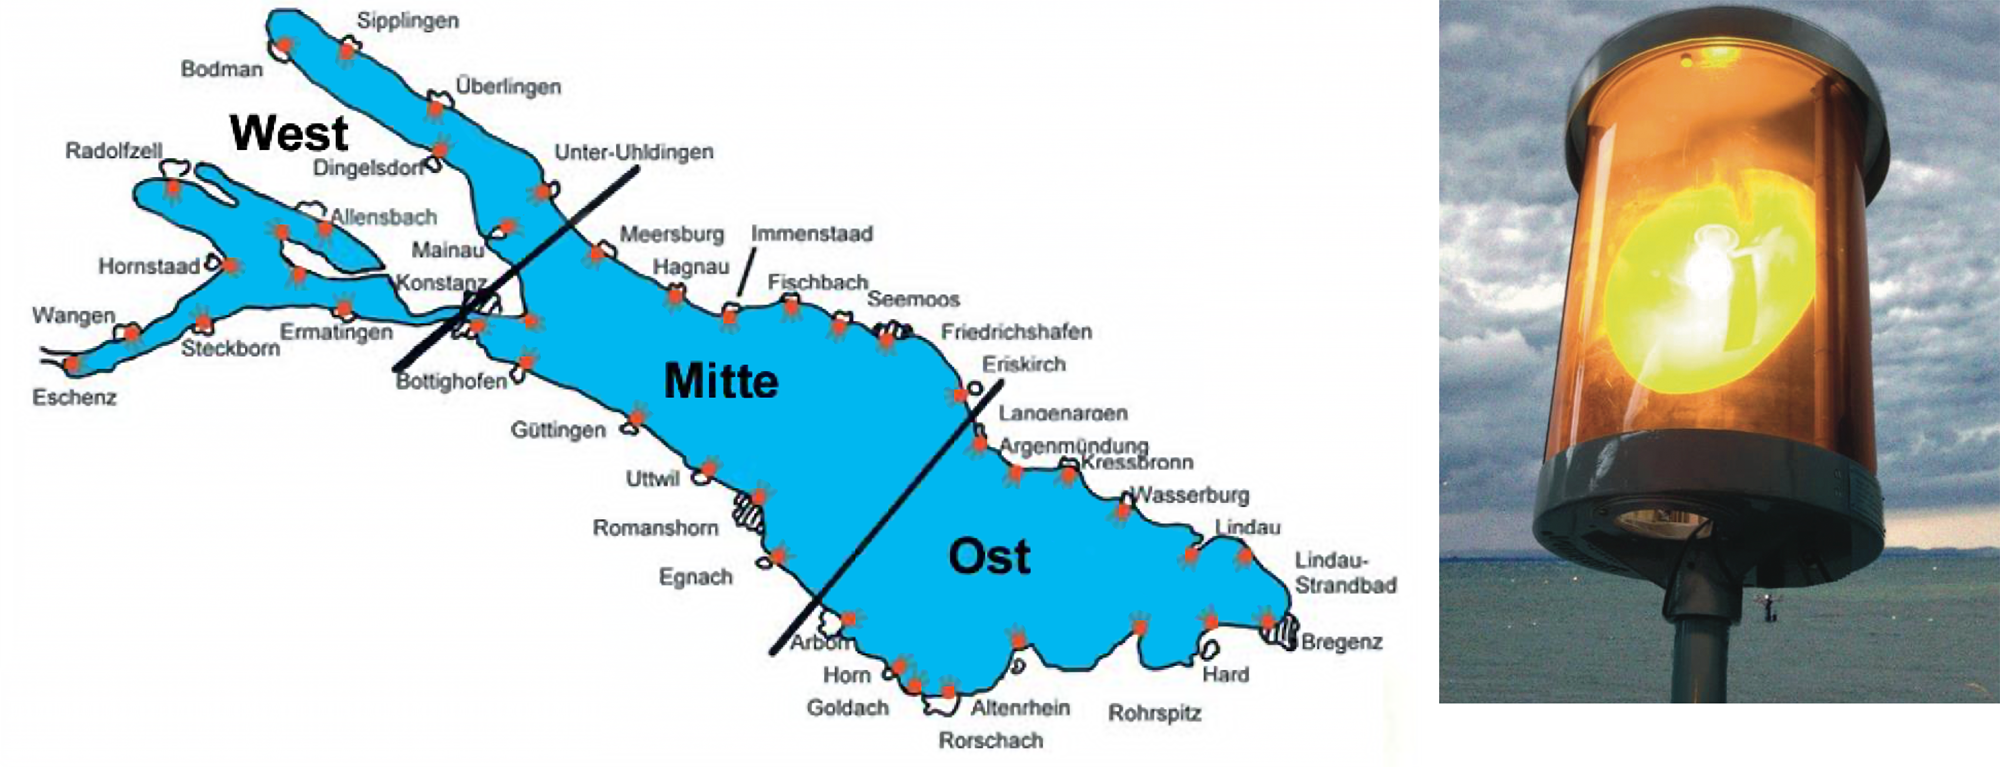
\includegraphics[width=\textwidth-2\fboxsep-2\fboxrule]{img/sturm2}}
	%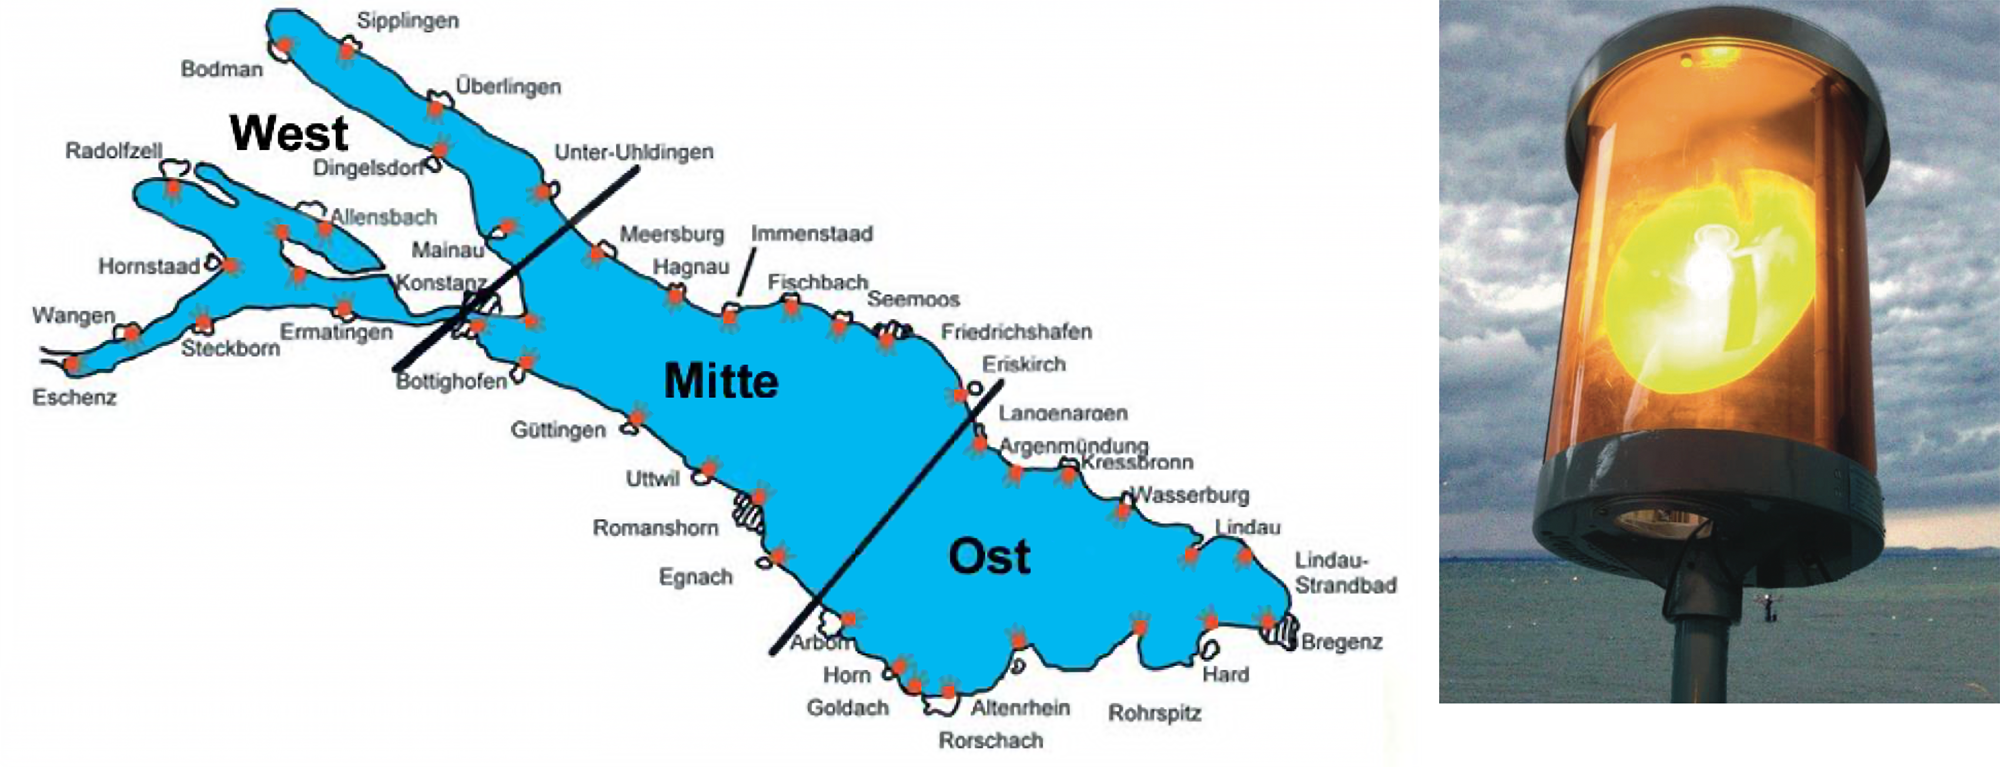
\includegraphics[width=1\linewidth]{img/sturm2}
	\caption{Sturmwarndienst Bodensee}
	\label{img:sturm2}
\end{figure}

% Problem: Kostenpflichtige Informaiton
Den aktuellen Status der Sturmwarnung kann sowohl beim Deutschen Wetterdienst, als auch bei meteoschweiz kostenpflichtig bezogen werden (ca. 1300CHF/Jahr). Kostenlos gibt es nur zwei browserkomatible Quellen: Das eine ist die allgemeine Mini-Warnkarte (173 x 109 Pixel) von meteoschweiz (siehe Abbildung \ref{img:sturm}, links) und das andere ist die Anzeige auf der Webseite der Kantonspolizei, Abbildung \ref{img:sturm}, rechts.

\begin{figure}[h!]
	\centering
  \fbox{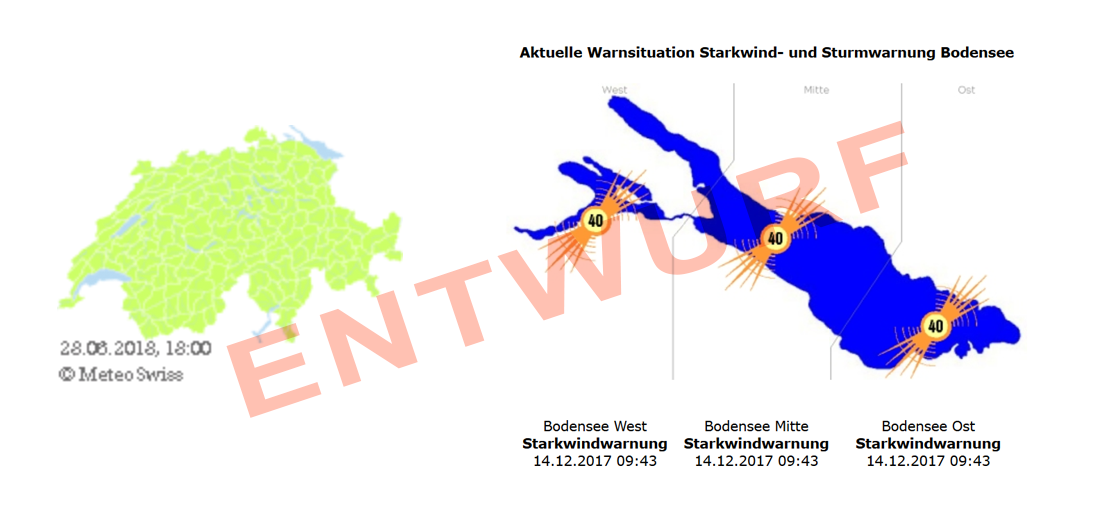
\includegraphics[width=\textwidth-2\fboxsep-2\fboxrule]{img/sturm}}
	%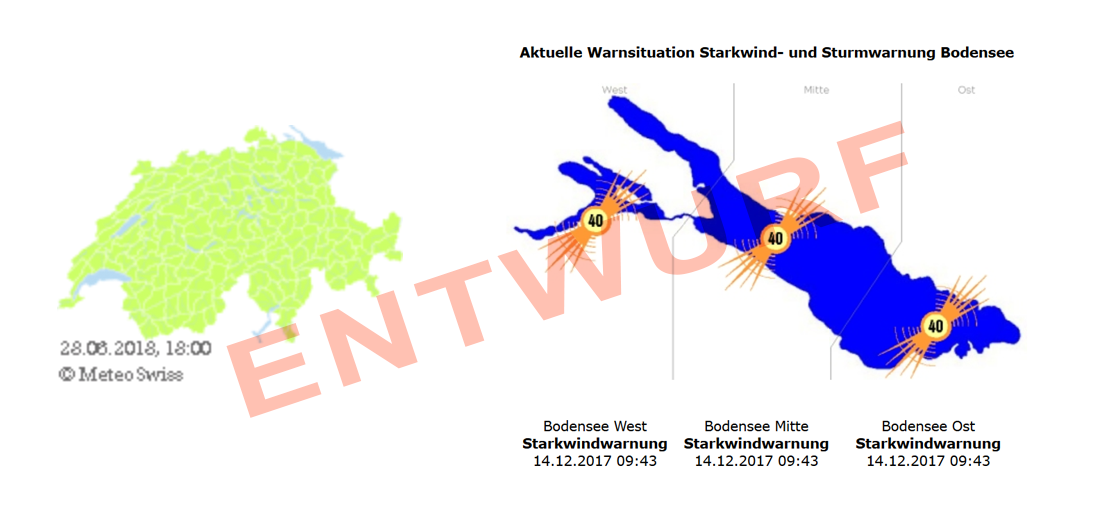
\includegraphics[width=1\linewidth]{img/sturm}
	\caption{Kostenlose Browserdarstellung}
	\label{img:sturm}
\end{figure}

Eine kostenlose API steht nicht zur Verfügung. Meteoschweiz verbietet es, Informaitonen von ihrer Website abzugreifen. Wir haben deshalb beim Amt für Informatik des Kantons Thurgau die Erlaubnis eingeholt, die Sturmwarndaten von der Kapo-Webseite abgreifen zu dürfen. Wir verwenden dazu die Python Bibliothek \textit{BeautifulSoup} als web crawler, wie in Listing \ref{lst:kttgCrawler} dargestellt. \newline

\begin{lstlisting}[label=lst:kttgCrawler,caption=Web Crawler für die Sturmwarndaten, language=python, style=py]
page = requests.get('http://www.kttg.ch/kapo/htm/stwarn.shtml')
soup = BeautifulSoup(page.text, 'html.parser')

# Einschaltzeit auslesen
soup.select('table tr:nth-of-type(4) td'):

# Status auslesen
soup.select('.titelfett strong'):
\end{lstlisting}

% Problem 1: keine API -> wenn Seite ändert, muss Crawler angepasst werden.
Das Problem beim Verwenden des Web Crawlers besteht darin, dass sobald die URL oder die Webseite geändert wird, der Crawler angepasst werden muss. Da der Crawler jedoch die einzige kostenlose Möglichkeit darstellt um die Daten zu erhalten, müssen wir dieses Risiko akzeptieren.

% Problem 2: Öffnungszeiten -> keine Warnung in der NAcht
Der Sturmwarndienst wie in Abschnitt \ref{subsec:sturmwarnung} beschrieben, ist kein 24h-Service. Der Dienst ist nur tagsüber aktiv zu den aufgelisteten Warnzeiten\footnote{ \url{https://kapo.tg.ch/public/upload/assets/56408/A5\%20Sturmwarnung.pdf}}, was aus Sicht der Sicherheit auf dem See nicht sehr sinnvoll ist.

\begin{itemize}
\item 1. April - 31. Oktober: 06:00 - 22:00 Uhr
\item 1. November - 31. März: 07:00 - 20:00 Uhr
\end{itemize}

\noindent
% Problem 3: rechtliche Verbindlichkeit der Sturmwarnung -> Zuverlässigkeit der anzeigen
Der Gedanke liegt nahe auf Grund der eigenen Windmessdaten eine Sturmwarnung anzuzeigen. In der Bodensee-Schifffahrts-Ordnung (BSO) Art. 6.13, steht jedoch:

\begin{quote}
\flqq Bereits bei Starkwind- und Sturmwarnung muss der Schiffsführer die durch die Umstände gebotenen Massnahmen treffen \frqq
\end{quote}

\noindent
 Da die Sturmwarnung auf dem Bodensee gesetzlche Pflichten mit sich bringt, haben wir uns entschlossen nur die offiziellen Daten anzuzeigen und nicht anderweitige Sturmwarnungen. Meteoschweiz bietet zudem auf ihrer MeteoSchweiz-App\footnote{ \url{https://www.meteoschweiz.admin.ch/home/service-und-publikationen/beratung-und-service/meteoschweiz-app.html}} die Möglichkeit von Push-Nachrichten bei Windwarnungen.




%-> Verweis auf Zeitungsartikel
%-> Meteoschweiz schickt in der Nacht keine SMS????? bzw. erstellt keine JSON????

% ins Kapitel API bzw. Cronjobs übernehmen
%Der Status der drei Teilabschnitte wird dann mintütlich in die Datenbank geschrieben. So kann der aktuelle Stand normal über die API abgefragt werden.

% nur im Vortrag erwähnen
% DAs JSON von Meteoschweiz kann leider nicht verwendet werden, da dessen URL bei jedem Update wechselt. Der genaue Pfad lässt sich nicht vorhersagen. Auf Grund des Zeitstempels lässt sich erahnen, dass es keine automatische Verbindung zwischen Meteoschweiz und den Sturmwarnleuchten am Bodensee gibt. Auf der Meteoschweiz-Seite ist z.B. der Zeitstempel 12:00 und auf der kttg.ch Seite 12:07. Wahrscheinlich erfolgt die Aktivierung manuell. Dies würde die Zeitdifferenz erklären.
% -> Foto Zeitstempel Meteoschweiz und kttg.ch
% Meteoschweiz leitet die Sturmwarnung an die Kantonspolizei Thurgau weiter. Diese schaltet die Sturmwarnung über eine eigne Software ein.



%% ###################################################################################################
%%   Unterkapitel
%% ###################################################################################################
\subsection{Grafische Darstellung der Wetterdatenverläufe}
\Diskussionspunkt{- Verwendetes JS-Framework (Chartist)}\newline
\Diskussionspunkt{- Welche Frameworks wurden betrachtet, warum ausgewählt?}\newline
\Diskussionspunkt{- Samplerate, fixe Y-Achse, Barrierefreiheit}\newline
\Diskussionspunkt{- x-Tage-Rückschau}\newline

Quelle: https://www.fusioncharts.com/javascript-charts-guide/

\subsubsection{Auswahl des JS-Frameworks}

1. Cross Browser Compatibility
It is a pain to handle cross-browser compatibility issues, and we believe the library you choose should do it for you.
Examples of libraries that work only on modern browsers: D3.JS, Chart.js and Chartist.js.
Examples of libraries that work in all the browsers: FusionCharts, amCharts and Highcharts.

2. Cross Device Compatibility
but if you want to ensure a consistent experience across hand-held devices as well, the charting library you choose should be responsive.
If you are making an application only for mobile, then you need to consider size of the library as well. This is because of lower processing power and browsing-speed issues in smartphones. A library with lower footprint is highly recommended in this case.

3. Input Data Format
Although JSON (JavaScript Object Notation) is gradually becoming the standard format especially when it comes to charting libraries. Most of the times you will have to load the data from a database like MySQL, Oracle or SQL Server. In this case you need to take into account the format which is acceptable to both your library and other parts of the application.

4. Customizability
This is one of the biggest decision factors for many. Is the charting library flexible enough so that you can make it do what you want, or will it just look good on defaults and you are on your own if you try to customize it?*
But with great customizability, comes great complexities. A good example of this is D3.js. It practically allows you to configure every element on the chart, but doing so is effort intensive. Then you have libraries like FusionCharts and Highcharts which strike a perfect balance between these two. Here you get a lot of freedom to customize your charts with minimum effort on your end.

5. Range of Available Charts
This one is a no brainer. Whatever visualization you want to create should be a part of the library. One useful advice here is that you should always consider your future needs as well and not just present ones.


6. Learning Curve
No doubt D3.js is very powerful, but if you are running on a tight deadline or using a charting library for the first time, it is not recommended to use D3.js.

7. Compatibility With Other Parts of Code OR Compatibility with Web-Frameworks
Imagine you are comfortable using PHP, ASP.NET, AngularJS or jQuery and are not familiar with vanilla JavaScript very much. Wouldn’t it be great if you can build charts using framework specific plugins or wrappers?

Some libraries have free plugins and wrappers that generate the required JavaScript and HTML code for you, which is then used to render charts on a web page.

8. Performance
If you have to plot fewer data points then most of the libraries will perform on a similar scale and you can neglect this factor. On the other hand if you have to render millions of data points, then performance becomes a major deciding factor as each fraction of second saved will have a huge impact in aggregate.

9. Exporting
It will be better that the charting library you choose supports export feature out of the box. Common export formats to look for are JPEG, PNG, PDF and SVG. There are two ways to export charts - client side and server side. Libraries like FusionCharts and Highcharts support both the ways of exporting. Only adding one line of code is enough to get this working.

10. Design and Interactivity
Design is more than just look and feel of a chart. It should not only look good (themes, color scheme), but it should have meaningful interactivity (hovering, click-through drill downs, live data updates, etc). For example, clicking a legend icon in multi-series line chart should toggle the visibility of related data plot. Custom code should not be required for that. Themes: another important design feature is the ability to theme your charts to match the design language of the rest of your application. A centralized theme manager - one place to manage the theming of your charts - will make your job much easier.


11. Community and Support
So when you face a problem, you might need some external support to solve it.

12. Accessibility
 does a charting library comply with 508 standards? Are screen readers like JAWS able to read the charts rendered by a library?

 WEbseite: http://accessibility.psu.edu/images/charts/
 jQuery Visualize: https://www.filamentgroup.com/lab/update-to-jquery-visualize-accessible-charts-with-html5-from-designing-with.html

13. Pricing and Licensing Terms
 Terms and pricing varies depending on factors like number of users, type of application (SaaS, intranet, web) and number of servers.

14. Open Source or Commercial
 Open-source is in fashion nowadays, but it’s not the right solution for every need.
 https://www.codeproject.com/Articles/581146/8-reasons-to-choose-commercial-library-instead-of



 D3 is an awesome javascript library, but it has no “ready to ship” charts and graphs.


\subsubsection{Vergleich Prognose/Ist Windgeschwindigkeit}

Die Messdaten der Wetterstation werden mit zwei Vorhersagediensten verglichen. Dabei wird jeweils die Eintages-Vorschau und die Dreitagesvorschau betrachtet.
Die Vorhersagedaten werden von den Anbietern nur in die Zukunft angezeigt d.h. wie die Vorhersage von gestern war ist nicht mehr ersichtlich. Aus diesem Grund müssen wir die Vorhersagedaten abgreifen und in unsere Datenbank speichern. Die Vorhersagen haben häufig einen Intervall von drei Stunden. Wir erstellen somit ein Skript, welche alle drei Stunden die Daten abfragt und speichert.

Die Darstellung von Vorhersage und Messresultaten erfolgt in einem Graphen, der den heutigen Tag, links davon die letzten 14 Tage und rechts davon die nächsten drei Tage anzeigt. Pro Anbieter und Prognoseart (1Tag bzw. 3 Tage) wird ein eigener Graph erstellt.

Diese Vergleiche werden aus reinem Interesse der IG erstellt und stellen keinen Service der IG dar. Die Wetterstation ist zudem windtechnisch eher an einem ungünstigen Ort platziert (Bucht), sodass die Messwerte nicht für den ganzen See representativ sind.
Aus diesen Gründen wird die Webseite zwar veröffentlicht, aber kein Link dazu auf der Webseite zur Verfügung gestellt.

Für den Prognoseanbieter haben wir uns für Openweathermap und windfinder entschieden. OWM bietet eine kostenlose Web-API. Windfinder ist eines der beliebtesten Seglertools, bietet aber keine API an. Dies Daten müssen somit aus der Windfinder-Webseite extrahiert werden.

Für die Darstellung der aktuellen Windgeschwindigkeit verwenden wir den Mittelwert der drei Werte aus der Stundenwert-Datenbank.

Openweathermap scheint sehr ungenaue Windvorhersagen zu liefern.

\Diskussionspunkt{-> Bild mit Vergleich von Messwerten, Vorhersage Windfinder und Vorhersage Openweathermap}\newline












%% ###################################################################################################
%%   Unterkapitel
%% ###################################################################################################
\subsection{Darstellung der historischen Daten}

\subsubsection{Daten der alten Wetterstation}
\Diskussionspunkt{- sind unbrauchbar weil.....}\newline
\Diskussionspunkt{- Grafik der Daten auf Zeitschiene}\newline
\Diskussionspunkt{- Pegeldaten (Excel)}\newline

\subsubsection{Daten der neuen Wetterstation}
\Diskussionspunkt{- Printscreen ungefiltert}\newline
\Diskussionspunkt{- Printscreen gefiltert}\newline

Die historische Daten sollen möglichst interaktiv gestaltet sein und ein aussagekräftiges Bild des Wetterverhaltens aufzeigen. Die historischen Daten liegen als Stundenwerte in der Datebank vor.
Tableau Public \footnote{ \url{https://public.tableau.com/de-de/s/}} ist ein Visualisierungsprogramm, das die Möglichkeit bietet direkt auf die Datenbank zuzugreifen. Die Visualisierungen sind einfach zu erstellen und interaktiv vom Benutzer filterbar.
Tableu Public ist kostenlos mit der Einschränkung, dass sämtliche Visualisierungen öffentlich sind. In unserem Fall ist dies kein Problem, da wir die Visualisierungen sowieso veröffentlichen. Um Visualisierungen veröffentlichen zu können ist ein Account nötig. Die Visualisierung kann anschliessend in die eigene Webseite eingebettet werden.

Für die Auswertung haben wir uns auf die Lufttemperatur, die Windrichtung und -geschwindigkeit sowie den Regen konzentriert.
Der Vorteil von Tableau ist, dass die Visualisierungen sehr einfach angepasst werden können wenn z.B. neue Messdaten hinzukommen. Tableau bietet auch die Möglichkeit Darstellungen für verschiedene Display-Grössen anzulegen. Da der Benutzer selbst keine Eingaben machen kann, sondern nur Filter setzen, ist die Gefahr von SQL-Injektion nicht vorhanden.


\subsubsection{Tableau Public}
\Diskussionspunkt{- Filtermöglichkeiten}\newline

% Nachteil 1: Keine direkte Verbindung zur Datenbank
Tableau Public\footnote{ \url{https://public.tableau.com/de-de/s/}} ist kostenlos, bietet jedoch keine Möglichkeit live auf die Datenbank zuzugreifen. Die historischen Daten müssen demnach manuell periodisch auf den Tableau-Server kopiert werden.\newline

%Nachteil 2: Nicht responsive -> Workaround nötig
\Diskussionspunkt{- Mobile Darstellunbg}\newline
\Diskussionspunkt{- Printscreen der mobilen Darstellung}\newline
\Diskussionspunkt{- Codesniplet auswahl desktop oder mobile}\newline

% Nachteil 3: nicht barrierefrei
\Diskussionspunkt{- Barrierefreiheit? Farben}\newline
\Diskussionspunkt{- Barrierefreiheit? Semantisches Web}\newline





%% ###################################################################################################
%%   Unterkapitel
%% ###################################################################################################
\subsection{Automatische Aktualisierung der Anzeigeelemente}
Die Wetterstation erzeugt jede Minute einen Datenbank-Eintrag mit den aktuellen Messwerten. Damit eine geöffnete Webseite immer auf dem aktuellen Stand ist, wird eine poll-Funktion verwendet, die selbständig alle 61 Sekunden von der API die aktuellen Werte abfragt wie in \ref{lst:poll} verkürzt dargestellt. Sobald die JSON-Daten eingetroffen sind, wird die Funktion \textit{updateData} aufgerufen, die wiederum die Anzeigeelemente und Texfelder aktualisiert. Die gesamte Aktualisierung wird asynchron mittels AJAX durchgeführt. Die Seite wird dabei nicht neu geladen, nur die Anzeigewerte. \newline


\begin{lstlisting}[label=lst:poll,caption=Automatische Aktualisierung der Werte, language=JavaScript, style=htmlcssjs]
(function poll() {
        $.get('https://api.wetter-arbon.ch/v1/')
          .done(function(response) {updateData(response);})
          .always(function() {setTimeout(poll, 61000); });
})();

function updateData(res){
        pressure_gauge.refresh(res.v1.data.pressure.value);
        $("#cwassertemp1m") = res.v1.data.watertemperature1m.value;
}

\end{lstlisting}


%% ###################################################################################################
%%   Unterkapitel
%% ###################################################################################################
\subsection{Barrierefreier Zugang}
Die Wetterstation und ihre Webseite ist eine Dienstleistung der Stadt Arbon. Sie gehört der Bevölkerung und soll deshalb für möglichst alle zugänglich sein. Sowohl die \flqq Web Content Accessibility Guidelines\frqq\footnote{ \url{https://www.w3.org/TR/2008/REC-WCAG20-20081211/}} des W3C-Konsortiums, als auch die deutsche \flqq  Barrierefreie-Informationstechnik-Verordnung\frqq\footnote{ \url{https://www.gesetze-im-internet.de/bitv_2_0/BJNR184300011.html}} bieten diverse Inputs, wie die Bedienbarkeit und somit Zugänglichkeit einer Webseite verbesserte werden kann.
\newline

\noindent
%\subsection*{Problem}
WeatherDisplay Live, welches zum Anzeigen der Wetterdaten verwendet wird, ist eine proprietäre Software, die nur sehr eingeschränkt angepasst werden kann und auf Adobe Flash basiert. Es lassen sich beispielsweise die Anordnung der Anzeigeelemente und die Einheiten konfigurieren. Viel mehr nicht.  Adobe Flash gilt als kritische Technologie in Hinblick auf Barrierefreiheit. Mit der jetzigen Konfiguration können die Anforderung an eine barrierefreie Seite nicht umgesetzt werde.
\newline

\noindent
%\subsection*{Lösungsansatz}
Wie in Abschnitt \ref{subsec:flash} erläutert, muss WeatherDisplay Live ersetzt werden. Das bietet die Möglichkeit, dass die Entwicklung der neuen Webseite nach den oben erwähnten Richtlinien erfolgen kann.

Von einer verbesserten Zugänglichkeit profitieren nicht nur Menschen mit Einschränkungen. Es geht darum, die Webseite so zu gestalten, dass sie möglichst für alle Benutzergruppen zugänglich ist. Dazu zählen nicht nur Menschen mit Einschränkungen. Auch veraltete Technik oder aber der allerneueste Stand der Technik können zu Schwierigkeiten führen. Ein hoher Lärmpegel (z.B. in einer Fabrikhalle) oder der Zwang zur Stille (z.B. in einer Bibliothek), der keine akustische Ausgabe gestatten oder Lichtverhältnisse, die einen besonders hohen Kontrast erfordern beeinflussen die Bedienbarkeit einer Webseite. Eine von Microsoft beauftragte Studie~\cite{ForresterResearch2004E:Abilities} der \flqq Forrester Research Inc.\frqq schätzt, dass über 60 Prozent aller Computernutzer von Barrierefreiheit profitieren können und gemäss \flqq Interface Design\frqq ~\cite{ThesmannStephan2016ID:U} wird Barrierefreiheit bald Standard sein.

Die aktuellen Web Content Accessibility Guidelines\footnote{ \url{https://www.w3.org/TR/WCAG20/}} fordern die Einhaltung von vier Designprinzipien:

\begin{itemize}
\item Prinzip 1: Wahrnehmbarkeit
\item Prinzip 2: Bedienbarkeit
\item Prinzip 3: Verständlichkeit
\item Prinzip 4: Robustheit
\end{itemize}

Die Ziele dieser vier Prinzipien sind durch zwölf Richtlinien genauer spezifiziert.

% Zu jeder Richtlinie geben die WCAG2 testbare Erfolgskriterien (Success Criteria) vor.

% Priorität 1 („Muss-Kriterien“): Webauftritte müssen alle A-Anforderungen erfüllen, weil es sonst für eine oder mehrere Benutzergruppen unmöglich wäre, auf die Information im Dokument zuzugreifen.

% Priorität 2 („Soll-Kriterien“): Die Erfüllung der AA-Anforderungen beseitigt signifikante Hindernisse und erleichtert einer oder mehreren Benutzergruppen den Zugriff auf Web-Dokumente.

% Priorität 3 („Kann-Kriterien“): Diese AAA-Anforderungen können erfüllt werden, um den Zugriff auf Web-Dokumente für eine oder mehrere Benutzergruppen zu erleichtern. Sind die Prioritäten 1 bis 3 erfüllt, erhält das Informationsangebot die Konformitätsstufe AAA.


Daraus ergeben sich folgende relevante Anforderungen für die Webseite der Wetterstation:


\subsubsection*{Wahrnehmbarkeit}
% Anforderung 1.1: Text-Alternativen
% Anforderung 1.2: Zeitbasierte Medien -> nicht relevant
% Anforderung 1.3: Anpassbarkeit
% Anforderung 1.4: Unterscheidbarkeit
Alle Nicht-Text-Inhalte, die dem Benutzer präsentiert werden, haben eine Textalternative, die dem entsprechenden Zweck dient.
Für die Darstellung der Seite muss CSS verwendet werden. Die einzelenen Blöcke müssen sematisch korrekt bezeichnet werden (RL 1.3)
Alle Nicht-Text-Inhalte, die dem Benutzer präsentiert werden, haben eine Textalternative, die dem entsprechenden Zweck dient.
Farbe ist nicht das einzige visuelle Mittel, um Informationen zu vermitteln, eine Handlung anzuzeigen, eine Reaktion auszulösen oder ein visuelles Element zu unterscheiden. ext kann ohne Hilfsmittel bis zu 200 Prozent vergrössert werden, ohne dass der Inhalt oder die Funktionalität verloren geht. Die visuelle Darstellung von Text hat ein Kontrastverhältnis von mindestens 7:1.
Für die visuelle Darstellung von Textblöcken steht ein Mechanismus zur Verfügung, um folgendes zu erreichen: (Level AAA)
Vorder- und Hintergrundfarben können vom Anwender frei gewählt werden.
Die Breite beträgt nicht mehr als 80 Zeichen oder Glyphen (40 bei CJK).
Der Text ist links ausgerichtet
Der Zeilenabstand (Vorspann) ist innerhalb von Absätzen mindestens anderthalb mal so groß wie der Zeilenabstand, und der Absatzabstand ist mindestens 1,5 mal so groß wie der Zeilenabstand.
Die Größe des Textes kann ohne Hilfsmittel bis zu 200 Prozent verändert werden, ohne dass der Benutzer horizontal scrollen muss, um eine Textzeile in einem Vollbildfenster zu lesen.

Interessante Farb-Auswahlwerkzeuge:
Colorchecker\footnote{ \url{http://accessible-colors.com}}
Colorsave\footnote{ \url{http://colorsafe.co}}
Colorbrewer\footnote{ \url{http://colorbrewer2.org}}


Problematisch ist die Kombination von Komplementärfarben, weil sie zu Flimmern führen können.~\cite{HellbuschJanEric2011Bvuu}

\subsubsection*{Bedienbarkeit}
% Anforderung 2.1: Zugänglichkeit per Tastatur
% Anforderung 2.2: Bereitstellung ausreichender Zeit
% Anforderung 2.3: Vermeidung von Anfällen
% Anforderung 2.4: Navigierbarkeit
Alle Funktionen des Inhalts sind über eine Tastaturschnittstelle bedienbar.
Webseiten enthalten nichts, was in einer Sekunde mehr als dreimal blinkt.
Der Zweck eines jeden Links kann aus dem Linktext allein oder aus dem Linktext zusammen mit seinem programmatisch festgelegten Linkkontext bestimmt werden. Es gibt mehr als eine Möglichkeit, eine Webseite innerhalb einer Gruppe von Webseiten zu lokalisieren. Überschriften und Labels beschreiben das Thema oder den Zweck. Jede Tastatur bedienbare Benutzeroberfläche hat eine Betriebsart, bei der die Tastaturfokusanzeige sichtbar ist. Informationen über den Standort des Benutzers innerhalb einer Reihe von Webseiten sind verfügbar. Abschnittsüberschriften dienen der inhaltlichen Gliederung.



\subsubsection*{Verständlichkeit}
% Anforderung 3.1: Lesbarkeit
% Anforderung 3.2: Vorhersehbarkeit
% Anforderung 3.3: Hilfestellung bei der Eingabe

Die voreingestellte menschliche Sprache jeder Webseite kann programmgesteuert bestimmt werden. Die menschliche Sprache jeder Passage oder Phrase im Inhalt kann programmatisch bestimmt werden, mit Ausnahme von Eigennamen, Fachbegriffen, Wörtern unbestimmter Sprache und Wörtern oder Phrasen, die Teil der Umgangssprache des unmittelbar umgebenden Textes geworden sind. Ein Mechanismus zur Identifizierung der erweiterten Form oder Bedeutung von Abkürzungen steht zur Verfügung.  Wenn eine Komponente den Fokus erhält, löst sie keinen Kontextwechsel aus. Wenn ein Eingabefehler automatisch erkannt wird, wird das fehlerhafte Element identifiziert und der Fehler dem Benutzer in Textform beschrieben. Labels oder Anweisungen werden bereitgestellt, wenn der Inhalt eine Benutzereingabe erfordert.  Wird ein Eingabefehler automatisch erkannt und sind Korrekturvorschläge bekannt, so werden diese dem Anwender zur Verfügung gestellt.  Es steht eine kontextsensitive Hilfe zur Verfügung.



\subsubsection*{Robustheit}
% Anforderung 4.1: Kompatibilität
 In Inhalten, die mit Hilfe von Markup-Sprachen implementiert wurden, haben Elemente vollständige Start- und End-Tags, Elemente werden entsprechend ihrer Spezifikationen verschachtelt, Elemente enthalten keine doppelten Attribute und alle IDs sind eindeutig.
